\chapter{Bilingual and multi-lingual baselines}

In this chapter, we describe the baseline experiments.
Bilingual baselines are needed to specify the starting point:
how good can a model perform on a specific translation direction
for each test set.

After bilingual results are collected and inspected, it is time for
multi-lingual baselines. For this purpose, we trained models
with randomly selected sets of target languages.
This way, we can see how much adding more target languages to the model
changes its performance on the same specific translation direction.

Most of the experiments are done on the \gls{en-to-36} dataset with
a couple of additional experiments on the \gls{en-to-5} dataset.


%----------------------------------------------------------------------
\section{\fix{Bilingual baseline}}
\label{section:bilingual_baseline}

We trained bilingual models on the \gls{en-to-36} dataset and received
a number of values for each translation direction, each value reflecting
the performance on a particular domain of the corpus.
Test results for relevant target directions (i.e. languages from
`Germanic' and `Slavic with Cyrillic script'
from Section \ref{subsection:proposed_experiments})
are shown in Table \ref{table:bilingual-results}.
For example, for \dir{En}{De} direction, we trained a bilingual model.
After that, we evaluated the model on the test set and received
\acrshort{bleu} scores for each sub-dataset, as shown
in \cref{fig:bilingual_en_de}.
Later, when an \dirmany{En}{De, others} model is trained and evaluated
on the same test set, its \dir{En}{De} performance on each sub-dataset
will be compared with these values.

\begin{figure}[h]
	\centering
	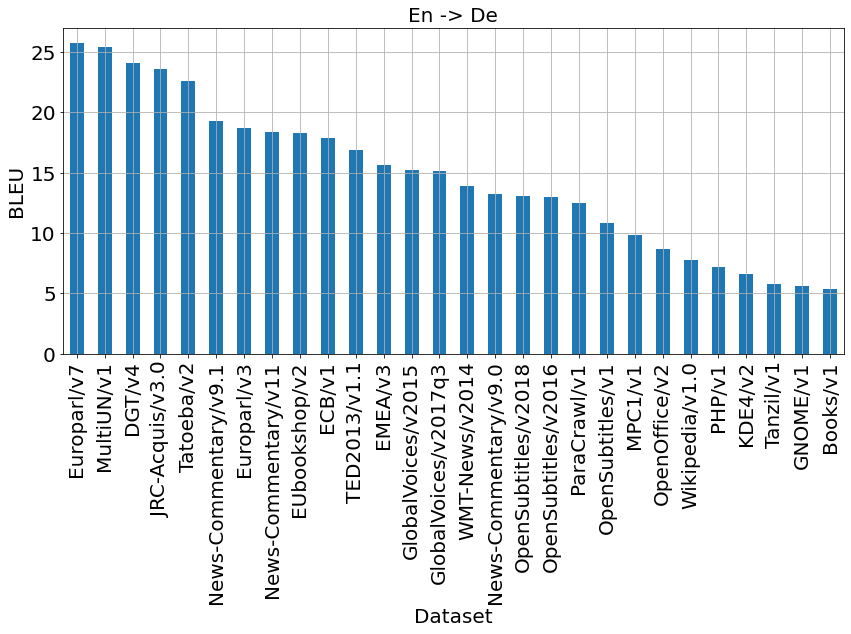
\includegraphics[width=0.9\columnwidth]{img/bilingual_en_de.png}
	\mycaption{\dir{En}{De} bilingual results}{
		Datasets on the $X$ axis are sorted by declining BLEU score.
		\fix{Color each column by dataset's group or add prefixes}
	}
	\label{fig:bilingual_en_de}
\end{figure}

In \cref{fig:bilingual_en_de} we can see that \acrshort{bleu} scores
for datasets in group 1 (\cref{tab:subdatasets_groups}), i.e.
Europarl/v7, MultiUN/v1, DGT/v4 and JRC-Acquis/v3.0 are the highest;
the lowest it is for sub-datasets from groups 4 and 5, such as
PHP/v1, KDE/v4, Tanzil/v1, GNOME/v1, and Books/v1.

BLEU score values for different test sets cannot be compared directly.
However, too big or too small value can give us some insight about the
data.

Let us look closer at some example translations from different
sub-datasets of the \dir{En}{De} test set.
In \cref{exmp:biling_de_europarl}, we can see a translation produced
by our bilingual \dir{En}{De} model compared with the reference translation
and two unnamed online translation systems.
The sentence pair is from the Europarl/v7 sub-dataset of
\dir{En}{De} test set.
As was stated in \cref{subsection:en-to-36}, Europarl/v7 was a prioritized
source of data to be sampled to the training set.
Even though our translation has different wording comparing to the reference one,
the sense is preserved.
Interestingly, at the same time, our translation is much closer
to the ones produced by online \acrshort{mt} systems.

\vspace{\baselineskip}
\begin{minipage}[t]{0.9\textwidth}

\textbf{Source (En):} \tagto{de}  Finally, I fully support the compromise agreement reached by our committee on Article 5 (4).

\textbf{Reference translation (De):}
Ich unterstütze ohne jede Einschränkung die von unserem Ausschuss
zu Artikel 5 Absatz 4 erzielte Kompromissvereinbarung.

\textbf{Our bilingual \dir{En}{De}:}
Schließlich unterstütze ich die von unserem Ausschuss erzielte
Kompromiss zu Artikel 5 Absatz 4 voll und ganz.

\textbf{OMT-G:}
Schließlich unterstütze ich voll und ganz die Kompromissvereinbarung,
die unser Ausschuss zu Artikel 5 Absatz 4 getroffen hat.

\textbf{OMT-D:}
Schließlich unterstütze ich voll und ganz die von unserem Ausschuss
erzielte Kompromissvereinbarung zu Artikel 5 Absatz 4.

	\begin{exmp}
	Bilingual \dir{En}{De} model's output of test set sentence
	translation (from Europarl/v7 sub-dataset)
	compared with the reference one and online
	translation systems OMT-G and OMT-D.
	Here and further for the online translation system, the target
	tag is omitted, and the target language is selected directly
	in the system.
	For our system, the following sentence is firstly preprocessed
	(see \cref{section:data_preprocessing}).
	\label{exmp:biling_de_europarl}
	\end{exmp}

\end{minipage}
\vspace{\baselineskip}


The next prioritized sources for sampling training data were
Eurobookshop and OpenSubtitles.
The first dataset has domain and vocabulary similar to the Europarl dataset.
OpenSubtitles dataset has data of a different domain:
transcribed human speech from films and series;
it has much shorter sentences and the speech of different register.

In \cref{exmp:biling_de_opensubtitles} we can see an issue of another kind
that might happen: a short sentence might not have all
the needed information. Here English `you' in the reference translation
translates as `ihr' (2. person, plural), and in our translation
as `Sie' (3. person, plural) which refers to a polite form of `you'.
One of the online \acrshort{mt} systems translates it as
`du' (2. person, singular).
The difference in exact translation of `you' affects the translation of
`know', because in German the verb has different conjugation for each
person and case, comparing to English, where s/es are only added
to the verb for 3. person, singular.

\vspace{\baselineskip}
\begin{minipage}[t]{0.9\textwidth}

\textbf{Source (En):} \tagto{de} Do you know it? 

\textbf{Reference translation (De):} Kennt ihr das?

\textbf{Our bilingual \dir{En}{De}:} Wissen Sie das?

\textbf{OMT-G:} Weißt du es?

\textbf{OMT-D:} Kennen Sie es?

	\begin{exmp}
	Example sentence from OpenSubtitles/v2018 sub-dataset of 
	the \dir{En}{De} test set.

	\label{exmp:biling_de_opensubtitles}
	\end{exmp}
\end{minipage}
\vspace{\baselineskip}

The main reason for introducing these detailed and domain-specific
baselines is that we want to make comparisons of BLEU scores as
reliable as possible.
Specifically, since different languages are differently covered by
the text domains, a single BLEU over a mixed test set would likely
hide important observations.

%----------------------------------------------------------------------
\section{\todo{Multilingual baseline}}
\label{section:multilingual_baseline}

Next after we have trained bilingual models and collected the results,
we trained multilingual baseline models -- the models with randomly
selected sets of targets.
We generated RANDOM task in a way we described in \cref{section:training_tasks}.

As we have seen in \cref{section:multitarget_theory}, models with more languages
in the mix usually perform slightly or significantly worse than bilingual ones.

However, there might be different unexpected effects due to slight domain-wise differences
in corpora content for different target languages.

\begin{figure}[h]
	\centering
	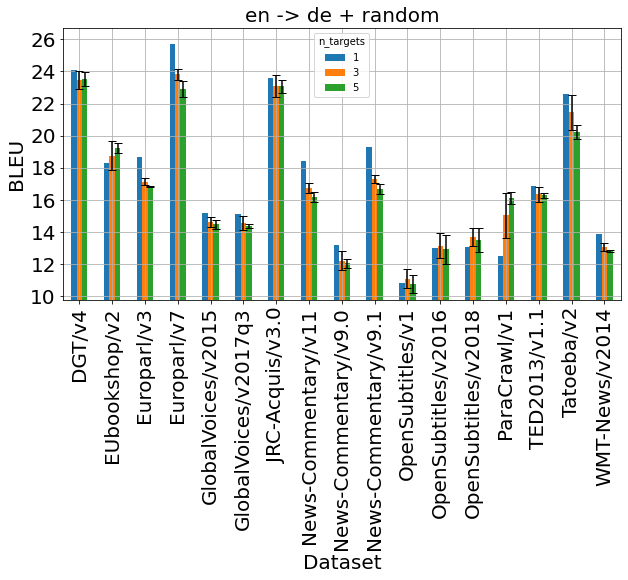
\includegraphics[width=1.0\columnwidth]{img/random_en_de.png}
	\mycaption{\dir{En}{De} multilingual baseline results (RANDOM)}{
		BLEU scores for \dir{En}{De} of multigarget models with
		randomly selected target languages and German as one
		of the targets.
		Datasets with BLEU lower than 10 are removed from
		this figure.
	}
	\label{fig:random_en_de}
\end{figure}

\todo{?}
When the size of the model is fixed, adding more translation directions usually causes
worsening of its performance.

\fix{refer to the table, explain, something like}
Across all considered configurations (e.g. English to 5 target languages),
there are too many specific settings how to conduct the experiment.
Already the choice of the particular languages offers too many setups
and we cannot afford to run them all.
We thus randomly sample and report the average BLEU and standard deviation
over all the particular runs we performed.
The actual number of runs is given in the column `count'.


\begin{table}[h!]
\begin{subtable}[t]{0.45\linewidth}
	\centering
	\begin{tabular}{rrrr}
	\toprule
	n\_targets &   mean &   std & count \\
	\midrule
	         1 &  41.40 &  ---  &   1 \\
	         2 &  40.60 &  0.20 &   3 \\
	         3 &  39.39 &  0.62 &   8 \\
	         4 &  39.40 &  0.71 &   2 \\
	         5 &  38.45 &  0.52 &   6 \\
	\bottomrule
	\end{tabular}

	\caption{
		En\to{}Bg for \emph{Europarl/v7} dataset.
		}
	\label{tab:bg/Europarl/v7}
\end{subtable}
\begin{subtable}[t]{0.45\linewidth}
	\centering
	\begin{tabular}{rrrrrrr}
	\toprule
	n\_targets &      mean &  std & count \\
	\midrule
	        1  &     19.50 &  --  &     1 \\
	        2  &     18.88 & 0.39 &     4 \\
	        3  &     17.45 & 0.52 &     4 \\
	        4  &     17.80 & 0.42 &     2 \\
	\bottomrule
	\end{tabular}
	
	\caption{
		En\to{}Ru for \emph{OpenSubtitles/v2016} dataset.
		}
	\label{ table:ru/OpenSubtitles/v2016 }
\end{subtable}
\mycaption{\acrshort{bleu} score change with adding target languages}{
    (a) First row: for mono-lingual En\to{}Bg model test \acrshort{bleu} score is 41.40.
    Second row: for 3 (column \emph{count}) En\to{}Any
    models with two target languages
    (column \emph{n\_targets}) one of which is Bulgarian
    the mean \acrshort{bleu} score is 40.60 with standard deviation 0.20.
    (b): same way as (a)
}
\end{table}



% \begin{table}[h]
% \centering
% \begin{tabular}{rrrrrrr}
% \toprule
% n\_targets & mean & count & std \\
% \midrule
%         1 &     --.-- &    1 &    -  \\
%         2 &     18.86 &    8 &  0.31 \\
%         3 &     17.59 &    8 &  0.48 \\
%         4 &     17.80 &    4 &  0.35 \\
% \bottomrule
% \end{tabular}
% 
% \caption{
% 	\acrshort{bleu} score for En\to{}Ru translation on test set part of
% 	\emph{OpenSubtitles/v2016} dataset.
% 	Description is the same as for table \ref{tab:bg/Europarl/v7}
% 	}
% \label{ table:ru/OpenSubtitles/v2016 }
% \end{table}


%----------------------------------------------------------------------
\section{\todo{Performance decrease on richer data sets}}
1 to 1, 2, 3 on UN corpus (much more sentence pairs per target language)

\begin{table}[h!]
\centering
\begin{tabular}{r|c}
\toprule
model         & BLEU  \\
\midrule
m.esfrru t.ru & 40.35 \\
m.esru t.ru   & 42.16 \\
m.frru t.ru   & 41.95 \\
m.ru t.ru     & 44.20 \\
m.esfrru t.fr & 45.03 \\
m.esfr t.fr   & 46.84 \\
m.frru t.fr   & 45.66 \\
m.fr t.fr     & 48.64 \\
m.esfrru t.es & 56.33 \\
m.esfr t.es   & 57.94 \\
m.esru t.es   & 57.31 \\
m.es t.es     & 59.94 \\
\bottomrule
\end{tabular}
\end{table}
